\subsection{Beam Photon Identification}\label{sec:analysis.beam}

As described in Sec.~\ref{sec:analysis.excluded}, only runs in which the beam current was 60-65~nA were used. This high current incident on the radiator can create multiple tagger hits within the time gate of the trigger. To determine which beam photon interacted with the target creating the event, a tagger time best matching the average \abbr{ST} time is chosen to be the time of the interacting photon that created the triggered event.

Due to the 2.004~ns \abbr{CEBAF} beam bunching spacing, there are possibilities in which a beam bunch will contain multiple bremsstrahlung photons that are indistinguishable in timing, within 2.004~ns, that satisfy the best tagger time. Figs~\ref{fig:beam.timing} and~\ref{fig:beam.timingII} show that $\simeq$ 86\% of events have a single in-time tagger-\abbr{ST} coincidence, $\simeq$ 11.5\% of events have two in-time tagger-\abbr{ST} coincidences, $\simeq$ 2\% of events have three in-time tagger-\abbr{ST} coincidences and $<$ .5\% of events have have more than three in-time tagger-\abbr{ST} coincidences. For the events in which there are multiple photons within the 2.004~ns window that are in time with the \abbr{ST}, the best photon is chosen at random with no preference to the energies of each photon. This method of random choice allows for a 7\% background increase due to the mismatching of the photon The 7\% is due to randomly choosing the incorrect photon $\frac{1}{2}$ of the 14\%. 

\begin{figure}[h!]\begin{center}
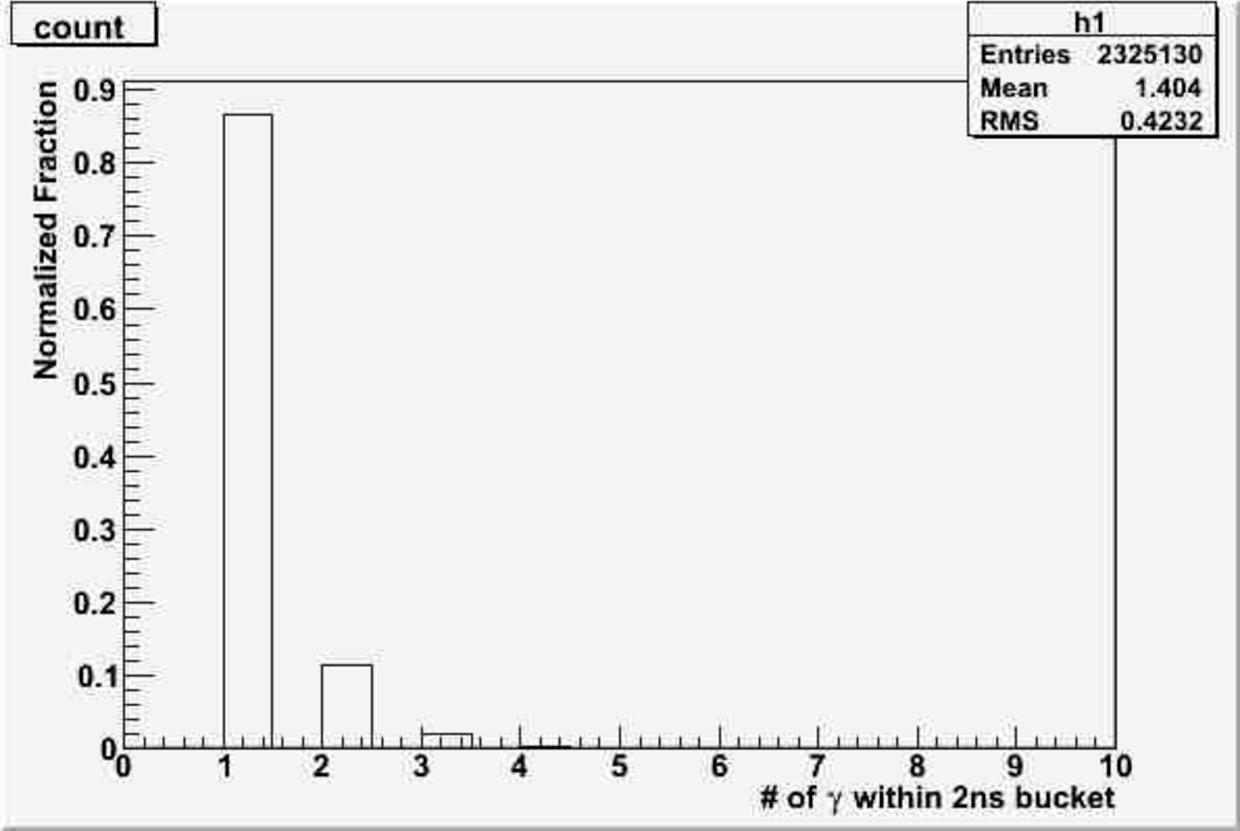
\includegraphics[width=\figwidth,height=0.75\hfigheight]{\figures/analysis/photon_timing/Photoncount1.pdf}
\caption[Probability of single and multiple photons within the \abbr{CEBAF} timing window of 2.004~ns]{\label{fig:beam.timing}Probability of single and multiple photons within the \abbr{CEBAF} timing window of 2.004~ns.}
\end{center}\end{figure}

\begin{figure}[h!]\begin{center}
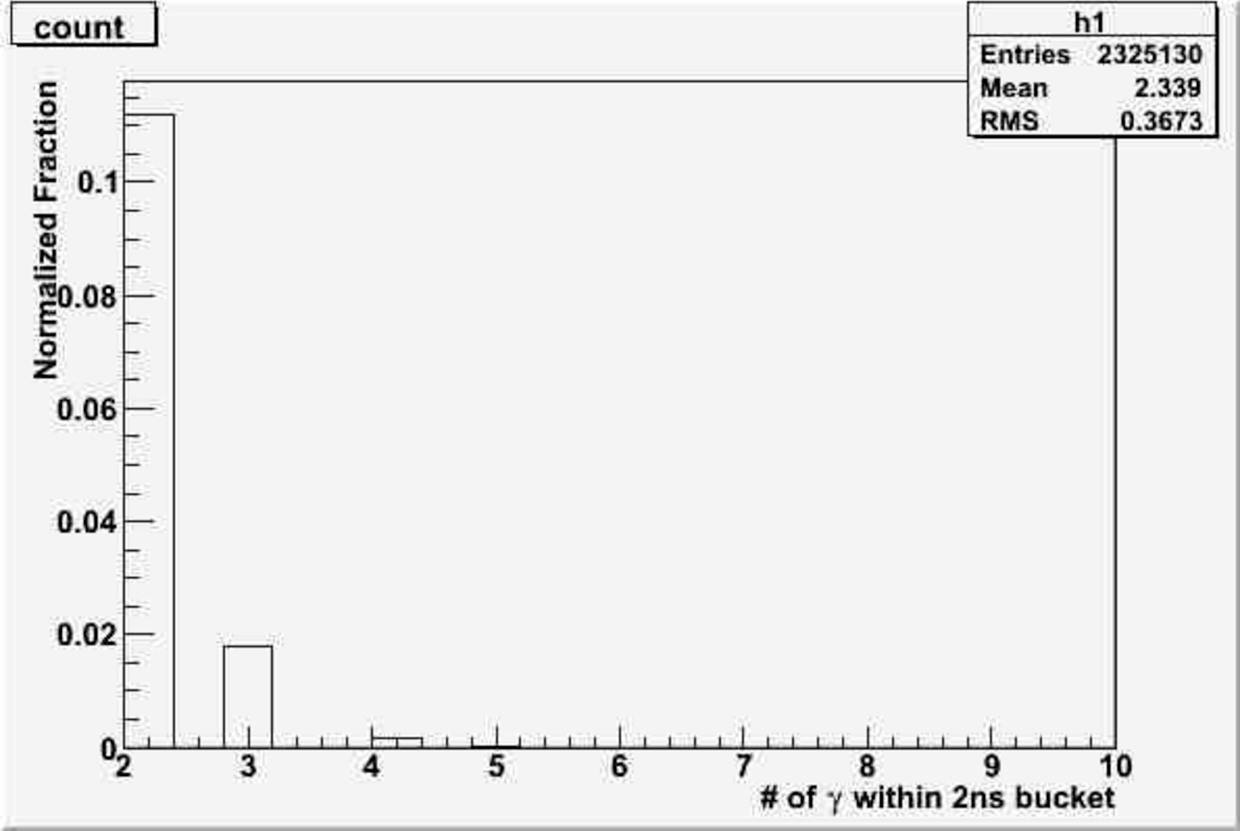
\includegraphics[width=\figwidth,height=0.75\hfigheight]{\figures/analysis/photon_timing/Photoncount.pdf}
\caption[Probability of multiple photons within the \abbr{CEBAF} timing window of 2.004~ns]{\label{fig:beam.timingII}Probability of multiple photons within the \abbr{CEBAF} timing window of 2.004~ns.}
\end{center}\end{figure}

\FloatBarrier